\section{ACOTH Inverse Hyperbolic Cotangent Function}

\subsection{Usage}

Computes the inverse hyperbolic cotangent of its argument.  The general
syntax for its use is
\begin{verbatim}
  y = acoth(x)
\end{verbatim}
where \verb|x| is an \verb|n|-dimensional array of numerical type.
\subsection{Function Internals}

The \verb|acoth| function is computed from the formula
\[
   \coth^{-1}(x) = \tanh^{-1}\left(\frac{1}{x}\right)
\]
\subsection{Examples}

Here is a simple plot of the inverse hyperbolic cotangent function
\begin{verbatim}
--> x = linspace(1,pi);
--> plot(x,acoth(x)); grid('on');
\end{verbatim}


\centerline{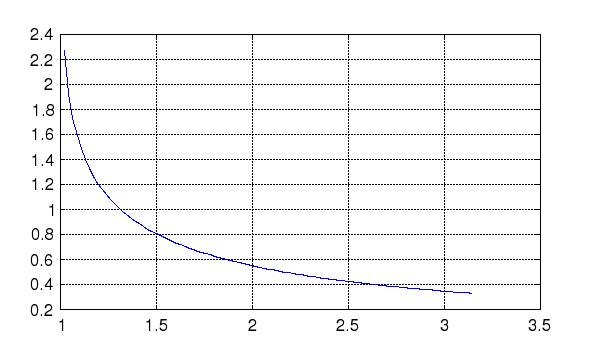
\includegraphics[width=8cm]{acothplot}}

